\section{Design and Implementation}
% General
% Describe how you have chosen to solve the problem
% Argue clearly for the choices made when designing and developing the solution.
The primary technique used for solving the problem of finding candidates of plagiarised documents has been the LSH algorithm and data structure. LSH has been chosen as it is an fast and space efficient algorithm which makes it ideal to perform a nearest neighbour search. Combined with other techniques, which will be described in the following, this solution has laid the foundation of the project.

\subsection{Modules}
% Introduce section
In this section the designed and implemented Python modules will be introduced, as well as reasoning for why certain design choices were made.

\paragraph{Wikiparser}
% Binary search to find location of article in index file.
% Decision to unzip small amount and process at a time.
% Remind what the size of the decompressed data is as a motivation to decompress on-the-fly
The \emph{Wikipedia} database is provided as a compressed archive of articles in the open-source \emph{bzip2} format with an accompanied index file listing the contents of the archive. Because the articles are formatted in XML and wikitext\footnote{A special markup language used by Wikipedia to format plain text into articles} the space of the compressed archive is significantly reduced. The sheer amount of data makes in infeasible to decompress and keep every article in memory. Remember that the archive is 16 GB compressed and 55 GB decompressed. We have circumvented this issue by performing an on-the-fly, as-needed decompression of articles while they are fed to the LSH algorithm. This reduces the necessary amount of memory to only keep a block (100 articles) in memory at a time. The operation is performed by reading the index file line by line, in which the start and end position of the data block can be found, then seeking and reading that block in the compressed archive file, decompressing and parsing the XML structure to separate articles. The implementation is achieved by overriding the \texttt{\_\_iter\_\_} and \texttt{\_\_next\_\_} methods from the \emph{Python} programming language to create an iterable object.

Another much needed functionality is fast lookup of articles. This is desirable because we quickly want to retrieve articles which has been marked as plagiarised. Because we have no intention to decompress the article archive and waste hard drive space, we want to perform the decompression on-the-fly. Since the index file is ordered by the article ID we can perform binary search and find the requested article in $\log(u)$ time. Although this binary search is mostly trivial, we have to take special care when seeking in the file since the position of file pointer is not guaranteed to be placed at the start of a new line. Following the binary search we can decompress the block and parse the XML as before.

\paragraph{LSH}
% The report does not discuss the benefits and downsides of LHS and what they mean for this project (compared documents have to be similar in length for it to detect candidates i.e).
% Benefits of using LSH

% Argue for the choice of parameters like q, r, b, k....
The LSH algorithm has a few different parameters, that should be set according to what you wish to achieve. One of them is the size of the shingles, $q$. For the matching of whole documents $q = 9$, as it is considered safe for large documents\cite{leskovec2014mining}. The remaining two parameters are $b$ and $r$, which are the number of bands and the number of rows in each band respectively. Choosing these parameters, will change the probability of the signatures in our data structure of becoming a candidate. With $b=20$ and $r=5$ we get the following curve as seen in figure~\ref{fig:lsh}. This gives us that when the similarity of two documents is $0.51$, then the probability of becoming a candidate is $>1/2$.

\begin{figure}[h]
	\centering
    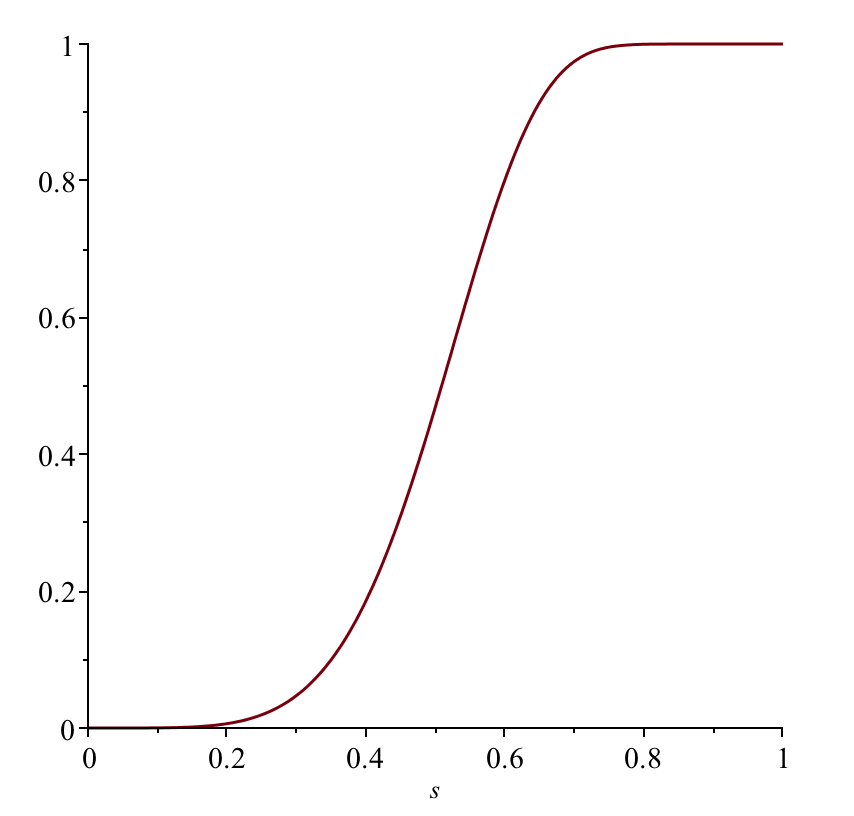
\includegraphics[width = 0.4\linewidth]{docs/report/input/lsh.png}
    \captionsetup{width = \linewidth}
    \caption{Probability of becoming a candidate versus Jaccard similarity of documents of choices of $b=20$ and $r=5$, $1-(1-s^r)^b$}
    \label{fig:lsh}
\end{figure}

\paragraph{Database}
% Show design of tables
% Argue why a database was used
% in Table 2 you have the same doc_id twice with different id. Is this the intended design?
Although LSH is a space efficient data structure and algorithm there is a trade-off between space and accuracy. Hashing many documents will inevitably grow beyond the amount what can be stored in memory. Storing the LSH data structure on disk will incur a performance penalty but will enable the data structure to grow in order of magnitudes larger than what can be fit in memory. We have chosen a database management system, specifically \emph{SQLite}, to store the LSH data structure. This is a nice abstraction because we can rely on the database for performance and optimisation of the queries. The design of the database schemes can be seen in figure~\ref{fig:schema}.\footnote{Created with: \url{https://github.com/schemacrawler/SchemaCrawler}} The database is comprised of two tables \emph{hashes} and \emph{documents} in which the attribute \emph{id} in \emph{documents} is a foreign key referencing the attribute \emph{id} in the \emph{hashes} table. This allows the database to only store the LSH band once and associate multiple documents to that band, thereby allowing a query to extract all documents associated with a band during a lookup for candidates. 

\begin{figure}[ht]
	\centering
    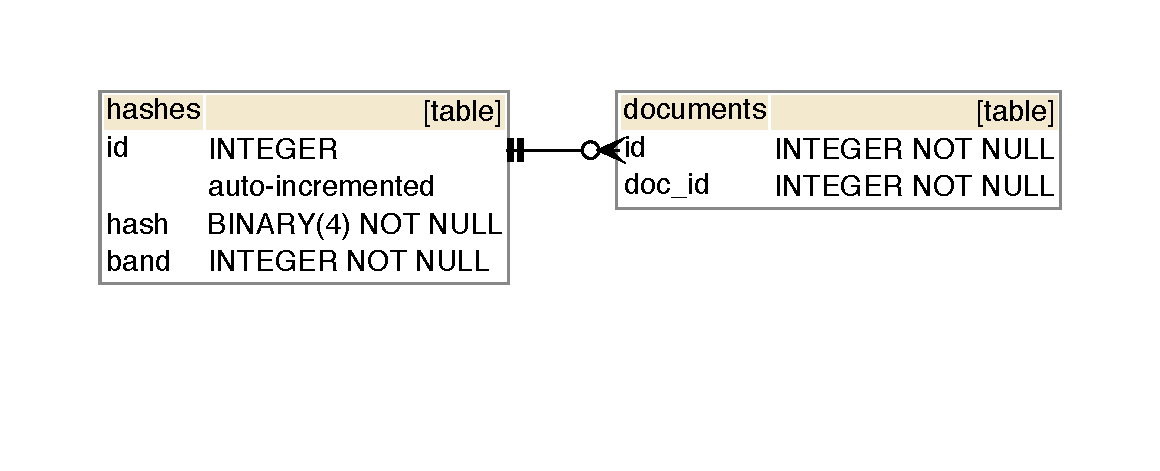
\includegraphics[width = 0.8\linewidth]{docs/report/input/schema.pdf}
    \captionsetup{width = \linewidth}
    \caption{Table \emph{hashes} which stores information on each LSH band with the hash value and the band id. Table \emph{documents} which associates documents with LSH bands from table \emph{hashes}.}
    \label{fig:schema}
\end{figure}

To assist with lookup performance both tables have indices on critical attributes. The \emph{hashes} table has a combined index on the \emph{hash} and \emph{band} attributes while the \emph{documents} table has an index on the the \emph{id} attribute alone. This is useful because an usual operation is the check of whether and band is already stored in the database, so as to only store it once. Both tables has a set of constraints such that no two identical bands can be stored and no article can be added to the same band twice, since this information is redundant.

\paragraph{MapReduce}
Using massively parallel computing we can distribute the work of computing signatures to multiple compute nodes. This is achieved through the popular \emph{MapReduce} processing technique. By using the \emph{Wikiparser} Python module we are able to output articles to \verb=stdout= which can then be piped into the \emph{MapReduce} worker implemented through \emph{mrjob}.\footnote{https://pythonhosted.org/mrjob/} The input is provided as seen in equation~\ref{eq:format} where the tab character is used to delimit the key/value pair.

\begin{equation}
    \textbf{[article\_id]}\textbf{\textless TAB\textgreater}\textbf{[article\_content]}\textbf{\textless NEWLINE\textgreater}
    \label{eq:format}
\end{equation}

The data flow of the \emph{MapReduce} operation itself can be seen i figure~\ref{fig:mapreduce}. Since every article is delimited by a newline character, articles are split out one document at a time. The mapper then splits the article into paragraphs and distributes them to different nodes. Since the article ID is used a key, all paragraphs from the same article will be processed on the same node. The reduce operation then calculates the signature for each paragraph and as a side-effect stores that information in the data base. The result is simply a key/value pair for every article which has been processed.

\begin{figure}[h]
	\centering
    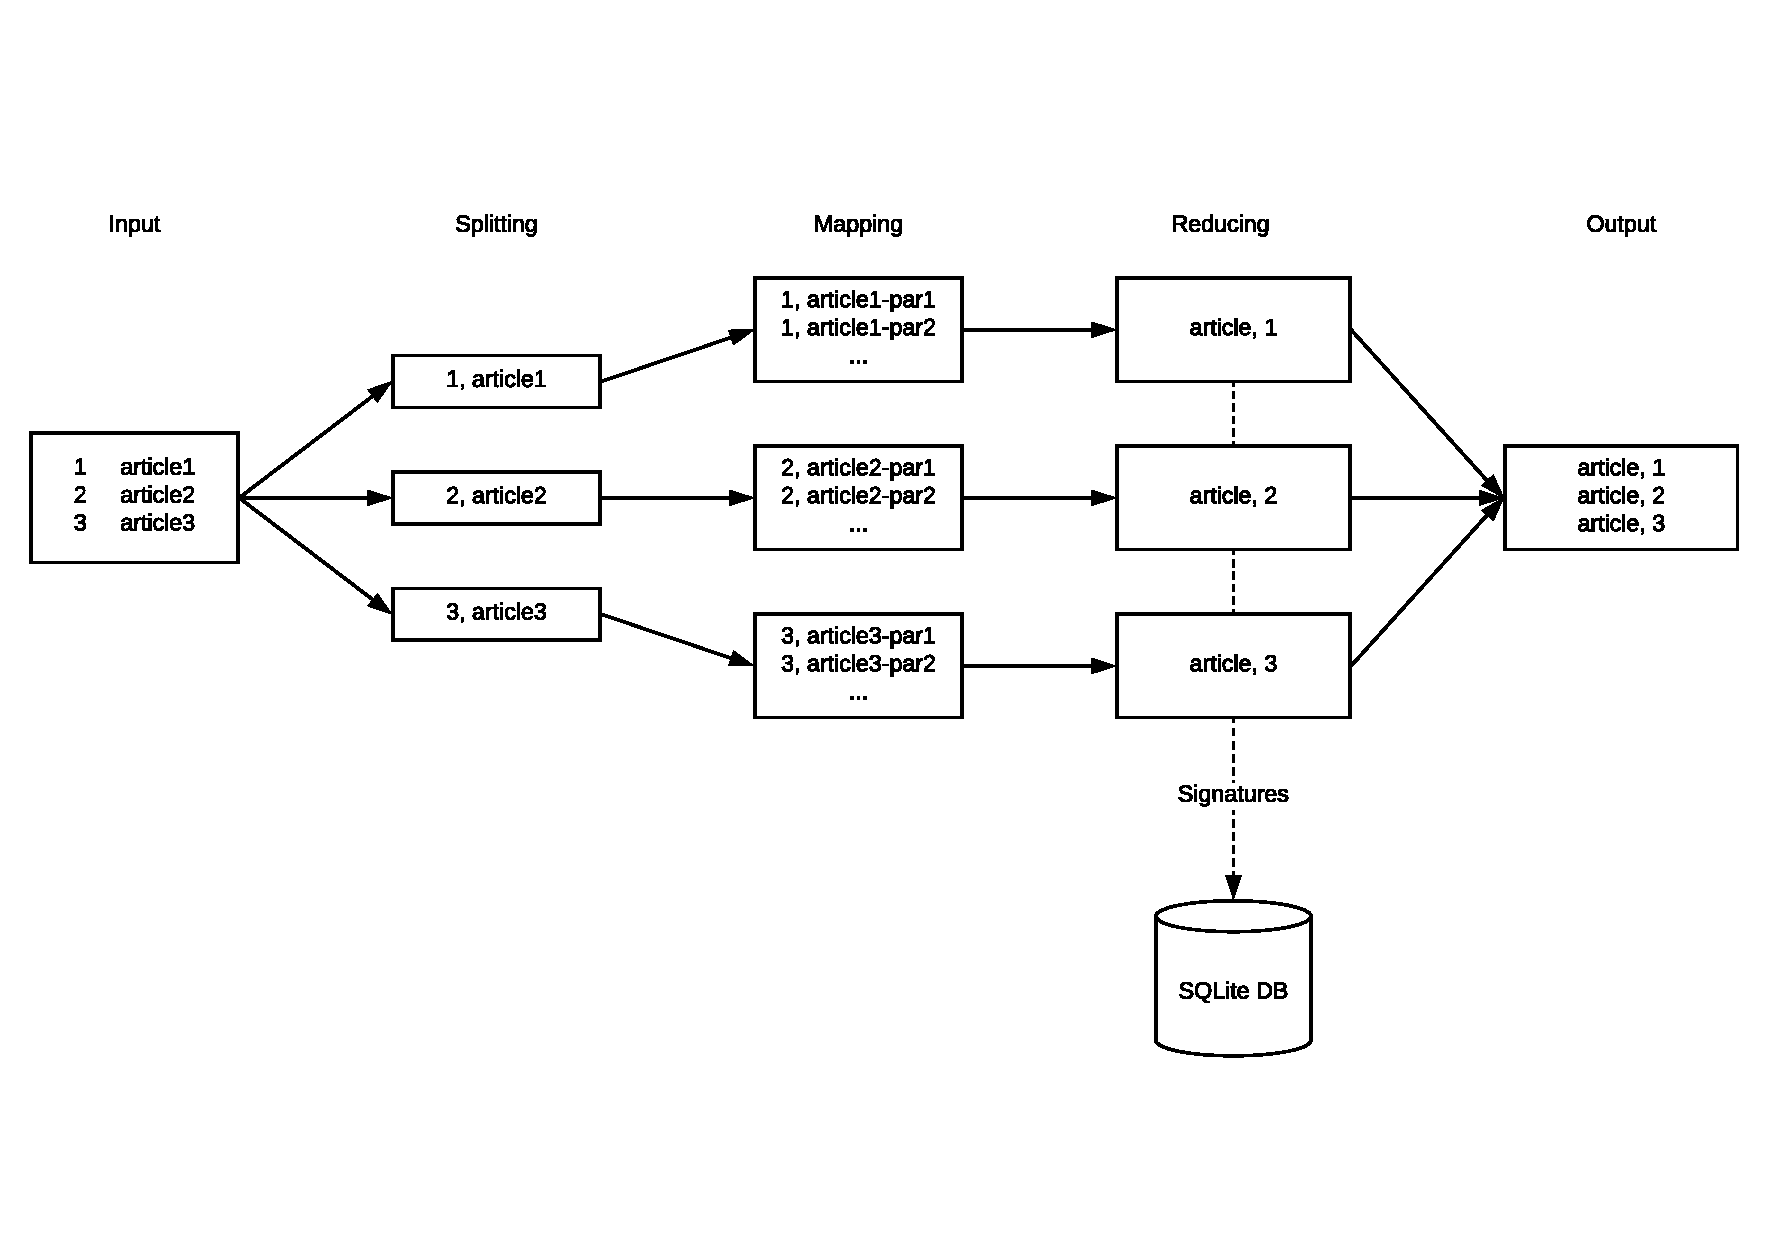
\includegraphics[width = \linewidth]{docs/report/input/mapreduce.pdf}
    \captionsetup{width = \linewidth}
    \caption{The MapReduce workflow of generating article signatures}
    \label{fig:mapreduce}
\end{figure}

Another similar but two-stage workflow is used to find candidates. Here the reduce operation performs a lookup in the data base instead, followed by stage 2 in which the reducer performs a set union on the candidates. The output is then a list of all unique candidates.

\subsection{Data processing}
The implemented solution offers two main operations, namely \emph{generate}, which will generate the data structure for a given number of Wikipedia articles, and \emph{lookup}, which will find the candidates from which a query documents could have been plagiarised from. These two operations will be described in the following. During both operations the content of the articles or the query document are cleaned. This cleaning is greatly inspired by the preprocessing and Natural Language Processing techniques that Chong et al. used.\cite{chong2010using}

\subsubsection{Generate}
\label{sec:gen}
The flow of the \emph{generate} operation can be seen in figure~\ref{fig:generate}. Here one can see that the \emph{generate} utilises the functionality implemented in the \emph{Wikiparser} and \emph{LSH} modules, as well as storing information in the \emph{Database}.

\begin{figure}[ht]
	\centering
    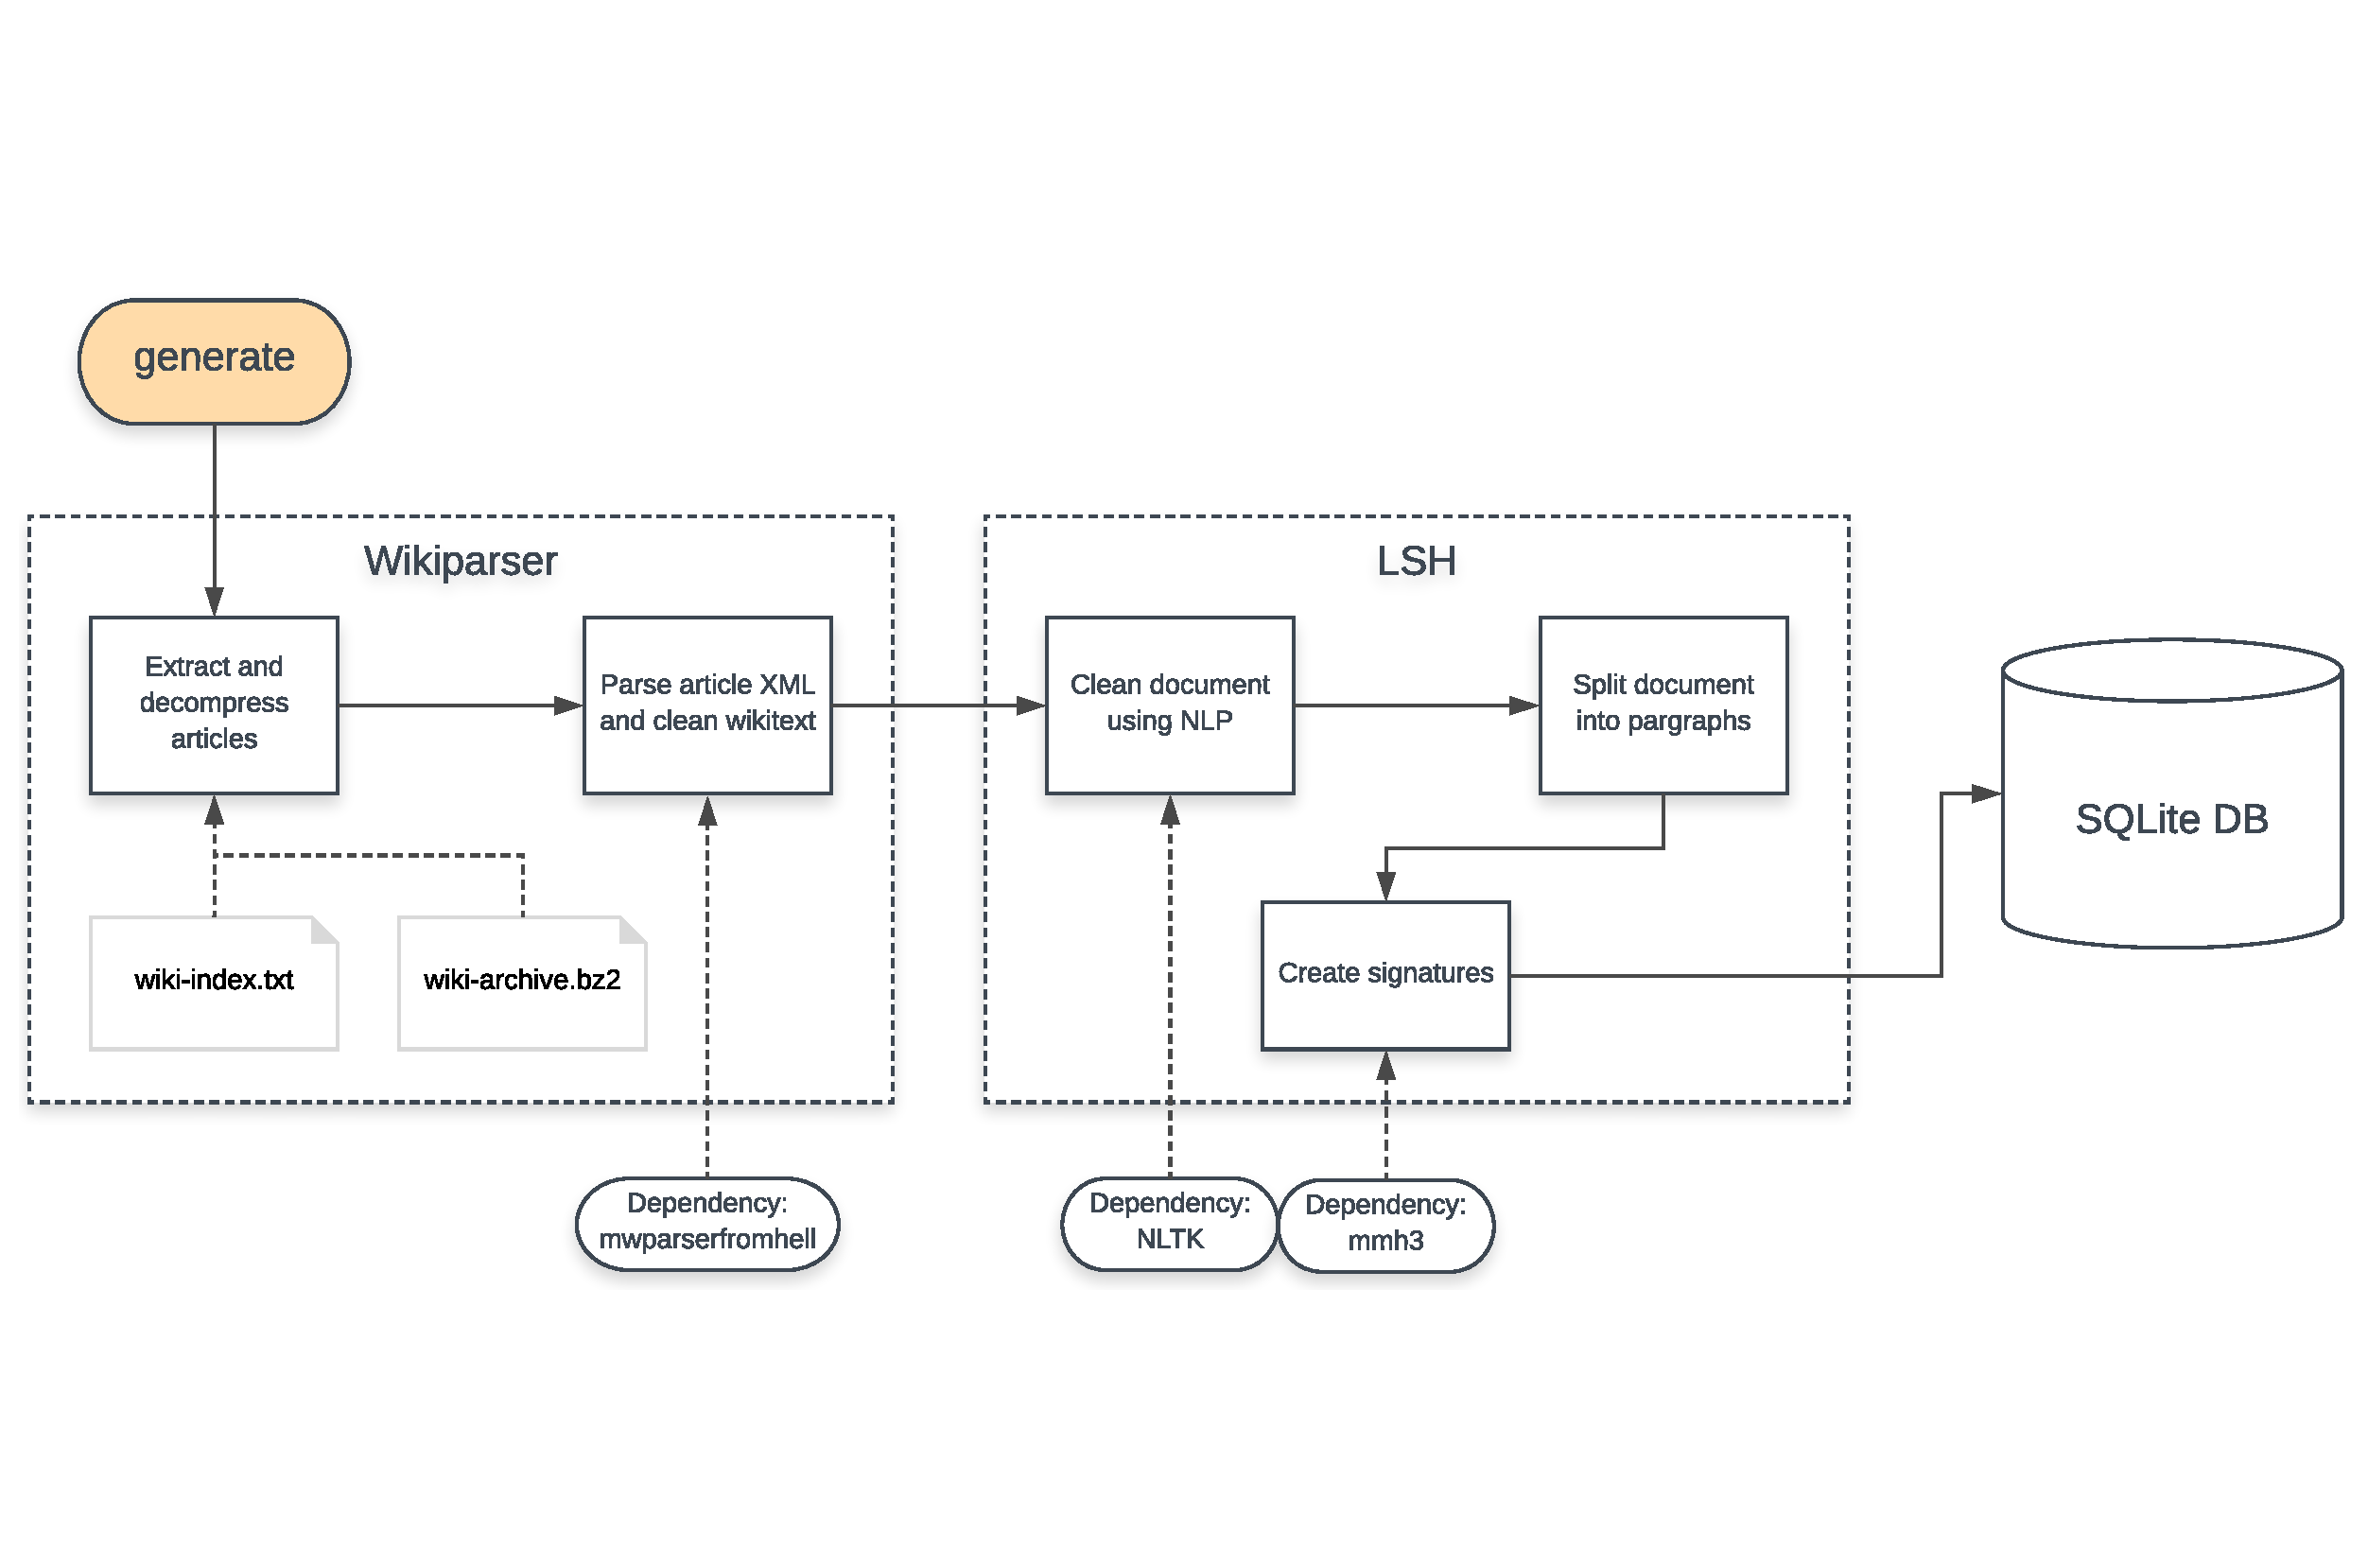
\includegraphics[width = \linewidth]{docs/report/input/generate.pdf}
    \captionsetup{width = \linewidth}
    \caption{Data flow of the \emph{generate} operation}
    \label{fig:generate}
\end{figure}

The general idea of the operation is as follows:
\begin{description}
    \item[Extract and decompress articles] The \emph{Wikiparser} will extract and decompress the articles. This will either be every Wikipedia article or a limited amount, depending on the given program arguments.
    \item[Parse article XML and clean wikitext] Each decompressed Wikipedia article will have the XML parsed and stripped of the wikitext markup, leaving only pure text.
    \item[Lowercase everything] To prepare the content of the article for having stop words removed, everything is transformed to lowercase. Furthermore this will ensure that no characters were changed by an adversary to lower- or uppercase to trick the algorithm, as this will affect the resulting hash value.
    \item[Remove stop words] To make the solution more robust against plagiarised content where minor changes have been made, all stop words are removed. Consider the following two sentences where a single word has changed: \say{This is \emph{a} test sentence of eight words}, \say{This is \emph{the} test sentence of eight words}. Hashing these two sentences will generate completely different hash values, but it is clear that they should be marked as plagiarised. This is avoided by removing the stop words as defined by NLTK\footnote{\url{https://gist.github.com/sebleier/554280}} and using the NLTK library\footnote{\url{https://www.nltk.org}}. Removing the stop words reduce both of them to \say{test sentence eight words}. The reduced sentences will now produce the same hash value and be detected as plagiarised correctly.
    \item[Remove special characters] As with stop words, where a small change in a sentence will result in a completely different hash value, the inclusion of special characters like \say{.}, \say{,}, \say{;} etc. will give a completely different hash value. For example the hash value of \say{example:} will not be the same as the the hash value of \say{example}. For this reason all special characters are removed from the content.
    \item[Replace all whitespace] To avoid creating shingles containing the \emph{empty string}, when passing the content to the LSH algorithm, all whitespace characters\footnote{\url{https://en.wikipedia.org/wiki/Whitespace_character}} are replaced with a single space. As the content of the documents are split by any whitespace character, consecutive whitespace characters would result in the empty string being added to the shingle. Furthermore is it not sufficient to simply split by the space character without removing the remaining whitespace characters, as they would then be part of the words after the split. The result of this would have a great influence on the generated hash value, e.g. \verb|split('two\t words') = ['two\t','words']|, where the tab character should obviously have been removed.
    \item[Split document into paragraphs] The document is then split into paragraphs of 80 words. A paragraph is considered to be around 125 words\footnote{\url{https://wordcounter.net/blog/2017/01/23/102485_how-many-paragraphs-is-1000-words.html}} but empirical data showed that removing stop words reduced the words in an article to $63\%$ of its original size, which gives $125 \cdot 0.63 \approx 80$. Each paragraph will overlap the previous paragraph by $50\%$. The reason being that if it was not overlapping, then an adversary would be able to place its plagiarised content such that it would only have a $50\%$ overlap with the paragraph it was plagiarised from in the data structure. This means that the Jaccard similarity of the adversary's paragraph will at most be $0.5$ and from figure~\ref{fig:lsh} one can see that the probability of being chosen as a candidate is then approximately $50\%$. Having each paragraph overlap the previous one in the data structure will increase the similarity to $0.75$ which increases the probability to approximately $1$.
    \item[Create and store signatures in database] Each paragraph for each article is then passed to the LSH algorithm, which will generate the signature and store it in the database.
\end{description}

\subsubsection{Lookup}
The flow of the \emph{lookup} operation can be seen in figure~\ref{fig:lookup}. Here one can see that the \emph{lookup} utilises a query document and the functionality implemented in the \emph{LSH} module, as well as retrieving information from the \emph{Database}.

\begin{figure}[ht]
	\centering
    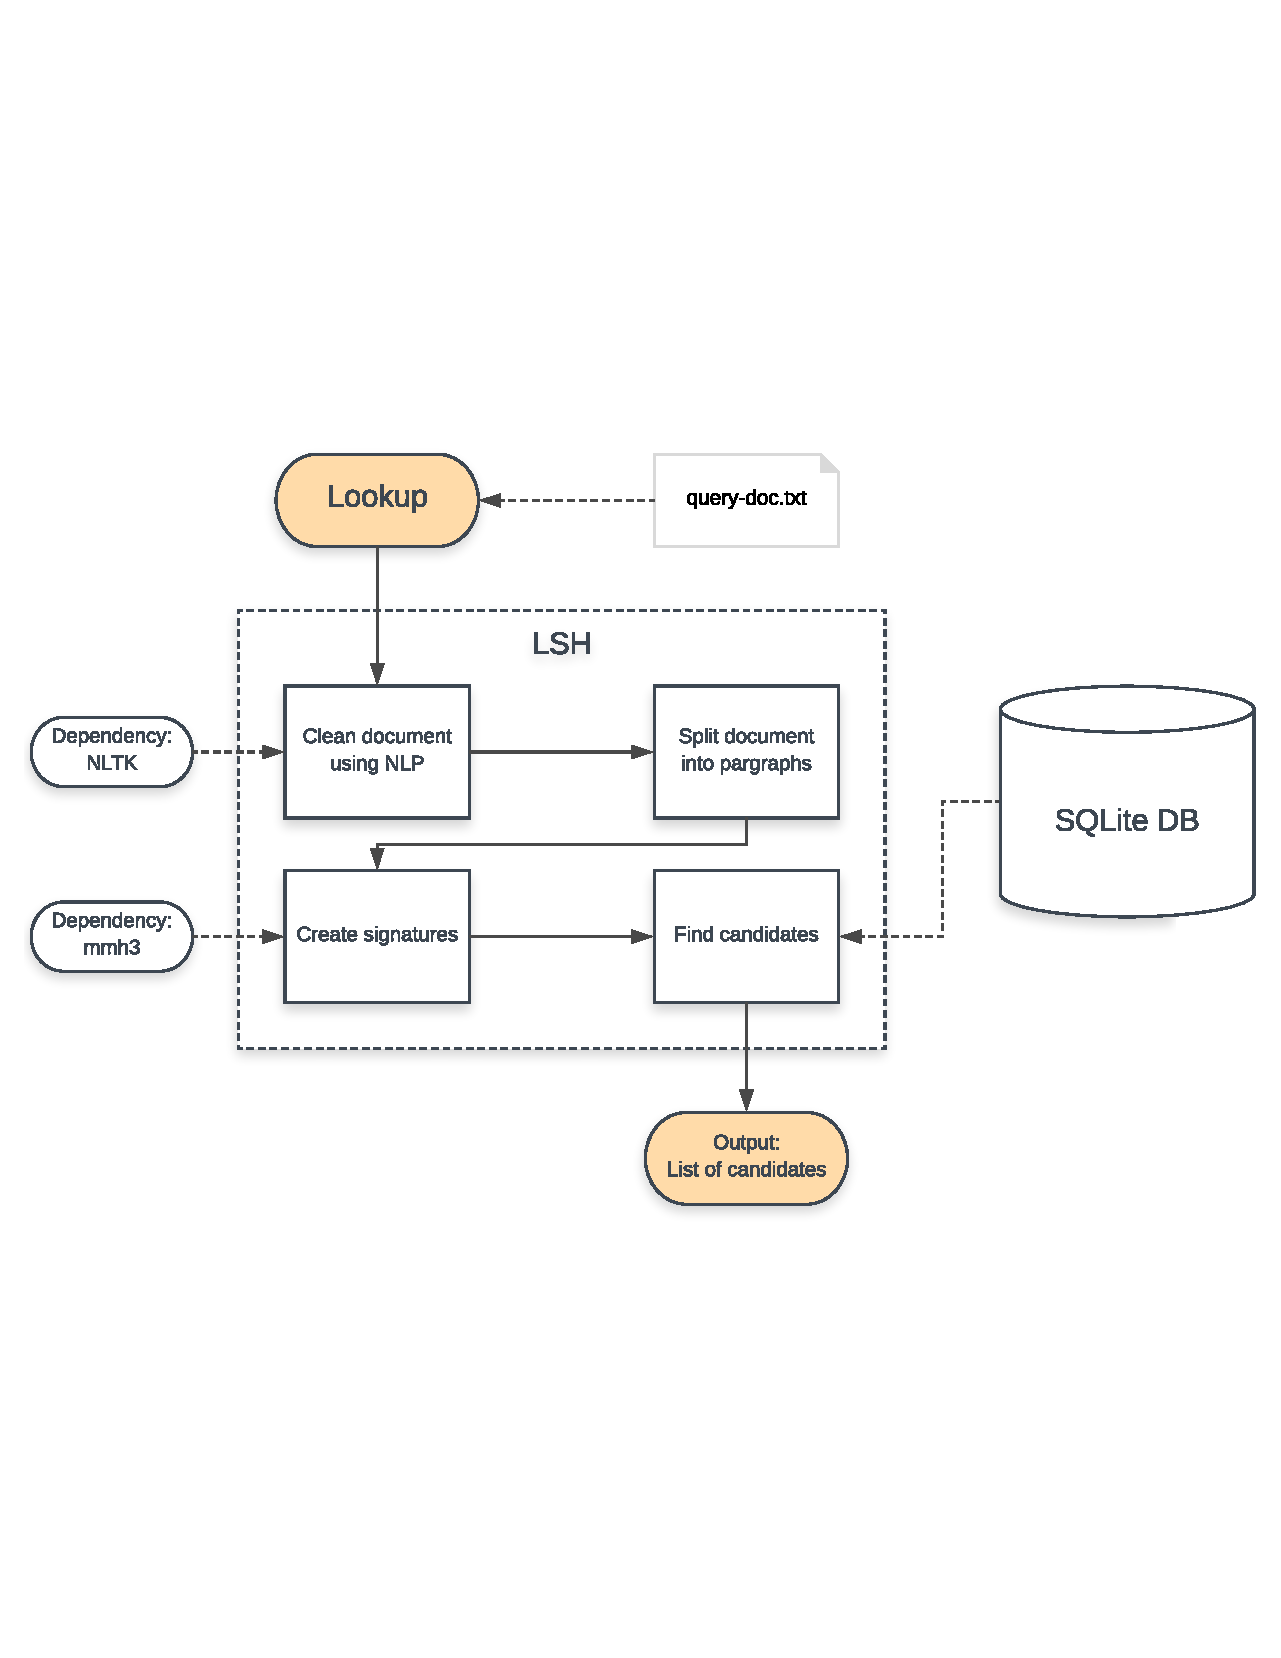
\includegraphics[width = \linewidth]{docs/report/input/lookup.pdf}
    \captionsetup{width = \linewidth}
    \caption{Data flow of the \emph{lookup} operation}
    \label{fig:lookup}
\end{figure}

\begin{description}
    \item[Prepare query document] The query document is prepared before the signature is generated by the LSH algorithm just like the articles were in the \emph{generate} process described in section~\ref{sec:gen}. That includes lowercase everything, remove stop words, remove special characters, replacing all consecutive whitespace characters with a single space character and splitting the document into paragraphs of the same size as during the \emph{generate} process.
    \item[Create signatures] When the preparation of the data content is complete the signatures of the paragraphs of the query document are generated. For this purpose the exact same LSH parameters as when the data structure was stored in the database has to be used.
    \item[Lookups in database to find candidates] The generated signatures are used to find matching hash values for the corresponding bands in the database. If a match is found, the article is considered a candidate and its article ID (stored under \emph{doc\_id} in the database) is appended to a list. When the signatures has been searched completely for possible candidates the list is returned to the user.
\end{description}